\documentclass{report}
\usepackage[margin=1in, paperwidth=8.5in, paperheight=11in]{geometry}
%Math packages%
\usepackage{amsmath}
\usepackage{amssymb}
\usepackage{amsthm}
%Spacing%
\usepackage{setspace}
\onehalfspacing
%Lecture number%
\newcommand{\lectureNum}{18}
%Variables - Date and Course%
\newcommand{\curDate}{February 13, 2017}
\newcommand{\course}{MATH 239}
\newcommand{\instructor}{Luke Postle}
%Defining the example tag%
%\theoremstyle{definition}%
\newtheorem{ex}{Example}[section]
%Setting counter given the lecture number%
\setcounter{chapter}{\lectureNum{}}
%Package for drawing graphs%
\usepackage{tikz}
\usepackage{verbatim}
\usetikzlibrary{arrows}

\begin{document}
%Note title%
\begin{center}
\begin{Large}
\textsc{\course{} | Lecture \lectureNum{}}
\end{Large}
\end{center} 
\noindent \textit{Bartosz Antczak} \hfill
\textit{Instructor: \instructor{}} \hfill
\textit{\curDate{}}
\rule{\textwidth}{0.4pt}
%Actual Notes%
\section{Matchings}
The final topic for graph theory.\\
A \textbf{matching} in a graph is a set of edges such that no two edges in the matching are incident with a common vertex.
\begin{ex}
A graph and its labelled edges $e_1$ and $e_2$ that are in a matching
\end{ex}
%Example 1%
\begin{center}
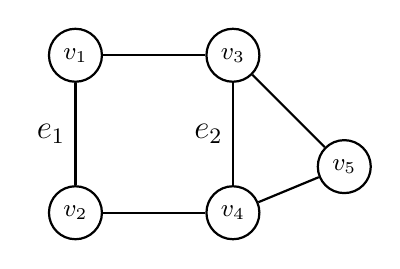
\begin{tikzpicture}[-,auto,node distance=2cm,
                    thick,main node/.style={circle,draw,font=\sffamily\small}]

  \node[main node] (1) {$v_1$};
  \node[main node] (2) [below of=1] {$v_2$};
  \node[main node] (3) [right of=1] {$v_3$};
  \node[main node] (4) [below of=3] {$v_4$};
  \node[main node] (5) [below right of=3] {$v_5$}; 
  
  \path[every node/.style={font=\sffamily\large}]
    (1) edge  node [left] {$e_1$} (2)
    	edge (3)
    (4) edge (2)
    	edge  node [left] {$e_2$} (3)
    	edge (5)
    (3) edge (5);
\end{tikzpicture}
\end{center}
Matchings can model trade deals, students and residencies, students and ``slots" in classes, etc. Now we'll look at a couple of definitions.
\subsubsection{Definition 1 | Maximum}
A matching $M$ or $G$ is \textbf{maximum} if there is no larger matching of $G$.
\subsubsection{Definition 2 | Saturated}
A vertex $v$ is \textbf{saturated} by a matching $M$ if $\exists \, e \in M$ incident with $v$ (\textbf{unsaturated} is the opposite). In example 18.1.1, $v_1, v_2, v_3, v_4$ are saturated; $v_5$ is unsaturated.
\subsubsection{Definition 3 | Alternating Path}
An \textbf{alternating path} $P$ of $M$ is a path in which every other edge is in $M$. In example, 18.1.1, $v_1v_2, v_2v_4, v_4v_3$ is an alternating path.
\subsubsection{Definition 4 | Augmenting Path}
An \textbf{augmenting path} $P$ of $M$ is an alternating path whose ends are unsaturated. This means that the first and last edge of an augmenting path are not in $M$. This implies that the number of edges in an augmenting path are \textit{odd}.
\subsection{Proposition 1}
\begin{center}
\textit{If P is augmenting, then $|E(P) \cap E(M)|<|E(P) - E(M)|$}
\end{center}
\subsection{Proposition 2}
\begin{center}
\textit{If P is an augmenting path of a matching M, and $M^\prime$ is obtained from M by switching the edges of P in M for the edges of P not in M, then $M^\prime$ is a matching}
\end{center}
\subsubsection{Proof of Proposition 2}
Every vertex of $P$ is in at most one edge of $M^\prime$, since the ends are unsaturated in $M$.
\subsection{Lemma 1}
\begin{center}
\textit{If M is a matching and P is an augmenting path of M, then M is not a maximum matching}
\end{center}
\subsubsection{Proof of Lemma 1}
Let $M^\prime$ be obtained from $M$ by switching on $P$. By proposition 2, $M^\prime$ is matching, yet $|E(P) \cap E(M)|<|E(P) - E(M)|$. Which leads to
$$|E(M)| = |E(M) \cap E(P)| + |E(M) - E(P)| < |E(M) - E(P)| + |E(P) - E(M)| = |E(M^\prime|$$ So $M^\prime$ is larger than $M$ and so $M$ is not maximum.\\
Actually, the converse of lemma 1 is also true (proof omitted), so the statement is actually an if-and-only-if:
\subsection{Lemma 1 (complete)}
\begin{center}
\textit{If M is a matching and P is an augmenting path of M if and only if M is not a maximum matching}
\end{center}
This implies that deciding if a matching is max is in co$-NP$. So we have a tool to show a matching is not maximum, but do we have a tool to show that is it?
\subsubsection{Definition 5 | Perfect Matching}
A \textbf{perfect matching} is a matching saturating every vertex. \textbf{Note:} not every graph has a perfect matching.
\begin{ex}
A graph with a perfect matching (edges in the matching are labelled $e_i$)
\end{ex}
%Eample 2%
\begin{center}
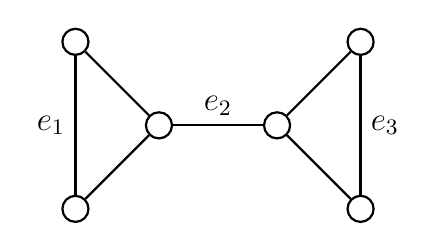
\begin{tikzpicture}[-,auto,node distance=1.5cm,
                    thick,main node/.style={circle,draw,font=\sffamily\small}]

  \node[main node] (1) {};
  \node[main node] (2) [above left of=1] {};
  \node[main node] (3) [below left of=1] {};
  \node[main node] (4) [right of=1] {};
  \node[main node] (5) [above right of=4] {}; 
  \node[main node] (6) [below right of=4] {}; 
    
  \path[every node/.style={font=\sffamily\large}]
    (1) edge (2)
    	edge (3)
    	edge node [above] {$e_2$} (4)
    (2) edge node [left] {$e_1$} (3)
    (4)	edge (5)
    	edge (6)
    (5) edge node [right] {$e_3$} (6);
\end{tikzpicture}
\end{center}
Our final tool for the day:
\subsubsection{Definition 6 | Cover}
A \textbf{cover} is a set of vertices such that every edge has at least one end in the cover (it's called a \textit{cover} because it represents a set of vertices that \underline{cover} all of the edges).
\begin{ex}
A graph with a cover (the vertices in the cover are labelled $m_i$)
\end{ex}
%Example 3%
\begin{center}
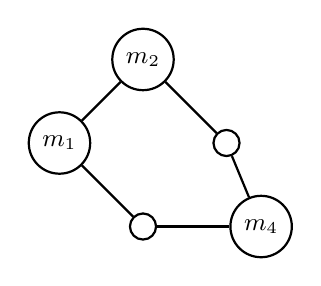
\begin{tikzpicture}[-,auto,node distance=1.5cm,
                    thick,main node/.style={circle,draw,font=\sffamily\small}]

  \node[main node] (1) {$m_1$};
  \node[main node] (2) [above right of=1] {$m_2$};
  \node[main node] (3) [below right of=1] {};
  \node[main node] (4) [right of=3] {$m_4$};
  \node[main node] (5) [below right of=2] {}; 
  
  \path[every node/.style={font=\sffamily\large}]
    (1) edge (2)
    	edge (3)
    (4)	edge (3)
    	edge (5)
    (2) edge (5);
\end{tikzpicture}
\end{center}
\subsection{Lemma 2}
\begin{center}
\textit{If M is a matching and C is a cover, then $|E(M)| \leq |V(C)|$}
\end{center}
\subsubsection{Proof of Lemma 2}
The cover $C$ has to cover all the edges of $M$ (i.e., $\forall \, e \in M$, at least one end must be in $C$). So $C$ has at least $|E(M)|$ vertices since no two edges of $M$ share a vertex, as desired.
\subsection{Corollary 1}
\begin{center}
\textit{The size of the max matching is less than the size of a min cover}
\end{center}
\subsubsection{Proof of Corollary 1}
If $M$ is a matching and $C$ is a cover, by lemma 2, $|M|\leq|C|$.
\subsubsection{Corollary 2}
\begin{center}
\textit{If M is a matching and C is a cover and $|M|=|C|$, then M is a max matching and C is a min cover}
\end{center}
\subsubsection{Proof of Corollary 2}
There can't be a larger matching $M^\prime$ because then $|M^\prime| > |M| = |C|$, a contradiction. Similarly, there can't be a smaller cover $C^\prime$ because then $|C^\prime| < |C| = |M|$, a contradiction.
\begin{center}
\textit{A question we'll look at next lecture is: when is the max matching equal to the min cover}
\end{center}
%END%
\end{document}